\begin{figure}[h!]
\centering
    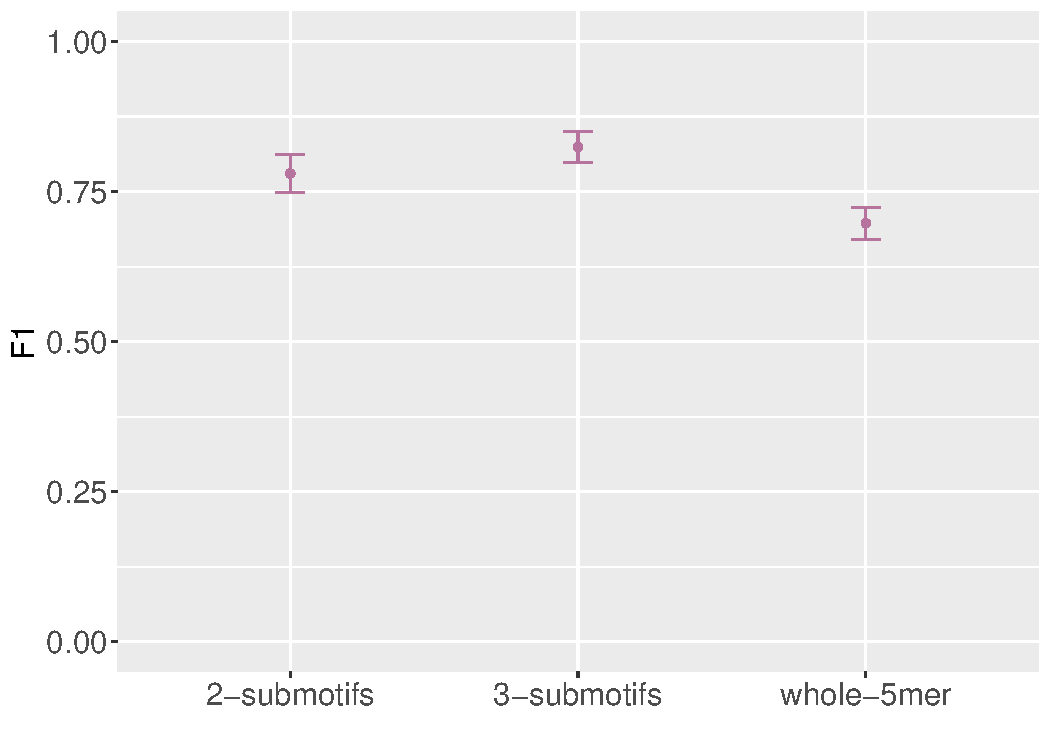
\includegraphics[scale=0.8]{graphics/f1_sce_submotif.pdf}
    \caption{\textbf{Dissecting 5-mer into multiple submotifs can potentially improve prediction accuracy compared to whole 5-mer}. For each combination of representation/metric, I iterated the training procedures of the KNN classifier 10 times using Jensen-Shannon distance. The performance of the classifier was computed based on a previously held out test data set and reported as confusion matrices and $F1$'s. The y-axis is the means of $F1$ for all representations, the error bars are the standard errors for the iterated $F1$’s.}
    \label{fig:f1_sce_submotif}
\end{figure}
